\section{Results: A Topological Crossover}\label{sec:results}

\subsection{An explicit star--slice crossover}

Proposition~\ref{prop:crossover} evaluates both competitors exactly at
$A(10,5)$, $R = 26$.  The strict inequality
$\SliceBoundary{} < \StarBoundary{}$ is an exact, order-independent statement:
both numbers are the cardinalities of the external-boundary sets of fixed
induced subgraphs.  It is the smallest explicit counterexample we know to the
prevailing assumption that hierarchical star subgraphs remain optimal as the
free-symbol count $m = n - k$ grows, and it marks the crossover at $m \ge 5$:
with more unused symbols available, an orthogonal hypercube embedding strictly
outperforms the prefix-ordered star.

\subsection{Geometric diagnostic}\label{subsec:trace}

To expose the mechanism behind the crossover, we track the marginal boundary
increment of each vertex as the two configurations are built under canonical
lexicographic insertion (Figure~\ref{fig:trace}).  We stress that the step-wise
increments are path-dependent: the trace is a structural diagnostic, not an
order-independent proof.  The endpoint values it reports, however, are
induced-subgraph boundaries and do not depend on the insertion order.

Under this ordering the binary slice takes the lead at the third vertex ($62$
versus $63$) and opens it to $76$ versus $82$ by the fourth, holding it through
$R = 26$.  The star exhibits a rigid block structure --- five successive
increments each of $+19$, then $+15$, $+11$, $+7$, $+3$ --- consistent with
saturating one coordinate fiber at a time, while the slice's increments decline
irregularly.  The star's early block growth is the local signature of its
single-coordinate construction: internal loops cannot close until an entire
branch has been saturated, so the marginal boundary cost stays high.

\begin{figure}[H]
	\centering
	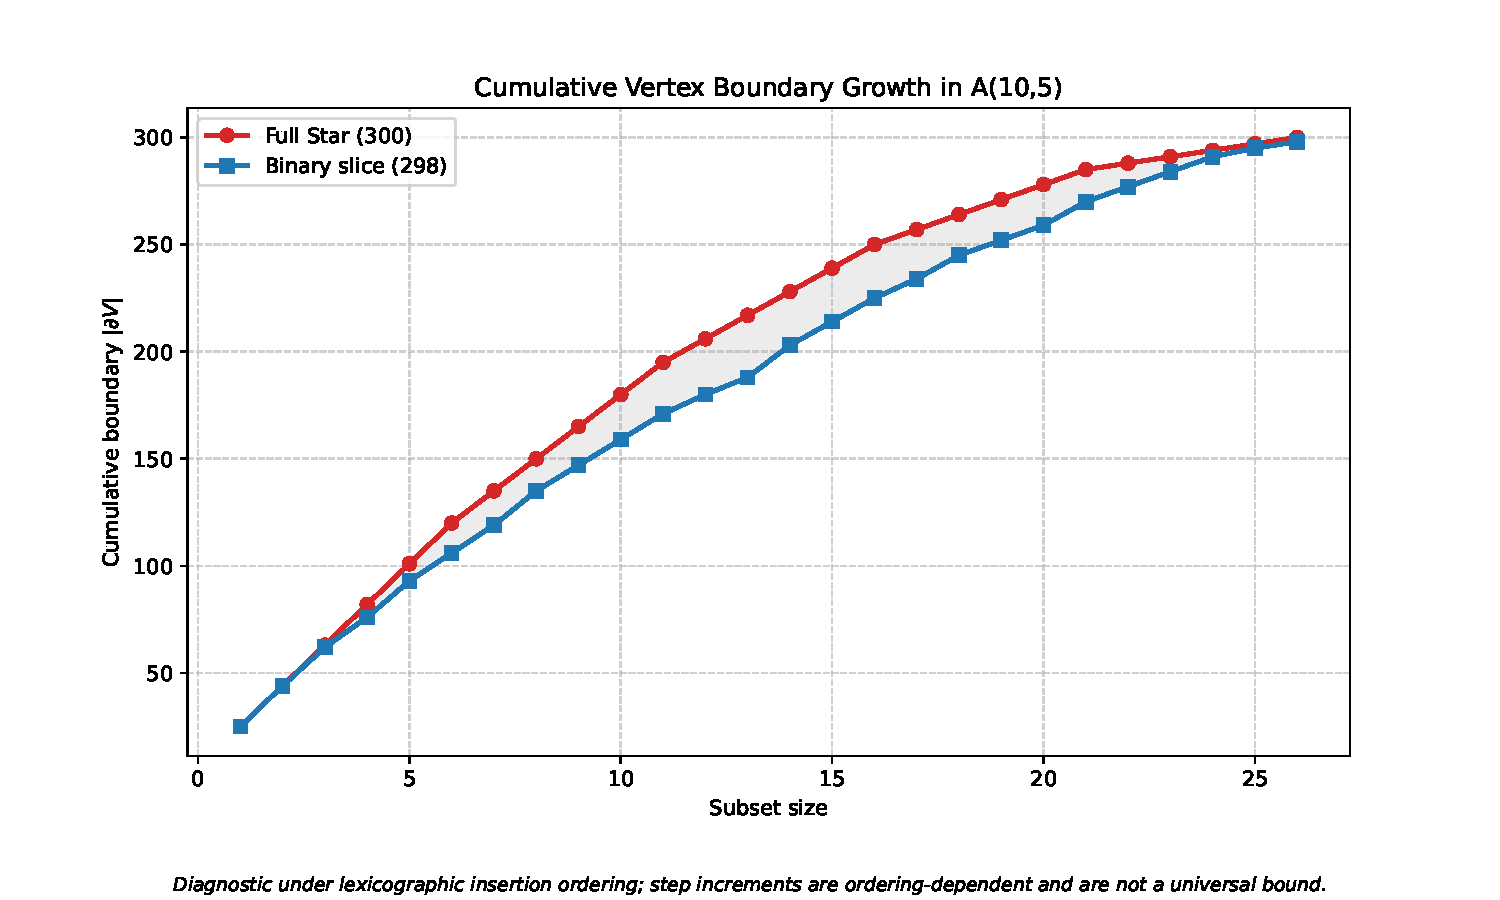
\includegraphics[width=0.9\textwidth]{../assets/out/boundary_diagnostic_plot.pdf}
	\caption{Cumulative external-boundary growth at $A(10,5)$ under
	lexicographic insertion.  The step-wise increments are path-dependent and
	serve as a diagnostic only; the terminal values ($\StarBoundary{}$ versus
	$\SliceBoundary{}$) are the insertion-order-independent boundaries of the
	two induced subgraphs.}
	\label{fig:trace}
\end{figure}

\subsection{CP-SAT certification}\label{subsec:cert}

The crossover supplies an upper bound; a lower bound requires an exhaustive
certificate.  Appendix~\ref{app:computational} gives the Boolean encoding:
binary variables $x_v, y_v$ per vertex, the volume constraint, and the boundary
implication, solved with the OR-Tools CP-SAT engine under an explicit symmetry
pin.  Because $A(10,5)$ is vertex-transitive, fixing one vertex in the subset
loses no minimum --- every $26$-subset is automorphic to one containing the
pinned vertex, and boundary size is invariant under automorphisms --- so the
certified floor is \emph{global}:
\[
	|\extbd(S)| \ge \CertFloor{} \quad\text{for every } S \text{ with } |S| = 26,
\]
and the true optimum is bracketed as
\[
	\CertFloor{} \le \min_{|S| = 26} |\extbd(S)| \le \SliceBoundary{}.
\]
We do not claim more: the search cutoff of $\HuntTarget{}$ (one below the
slice) has so far produced no feasible witness, so $\HuntTarget{}$ remains a
search target rather than a certified upper bound.
